\section{Statistical Learning}
Es existieren zwei grundlegende Arten von Statistischem Lernen. Regression, welche häufig für das Vorhersagen von zB Zeitlichen Ausgängen verwendet wird und Klassifizierung, um anhand eines Eingangs eine Klasse zuzuweisen.
\begin{center}
	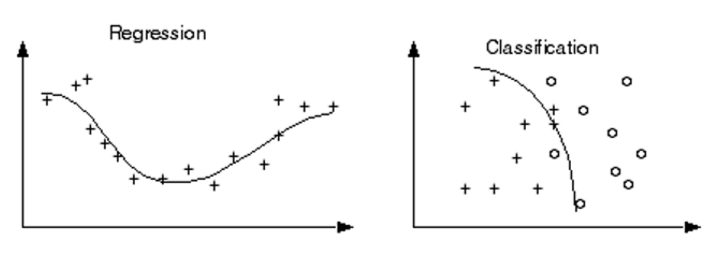
\includegraphics[width=\columnwidth]{./Images/types}
\end{center}

Um die Leistung der Vorhersage auf trainigsdaten zu bestimmen, wird zB Mean Squared Error verwendet \script{29}:
\[
MSE = \frac{1}{n}\sum_{i=1}^{n}(y_i - \hat{f}(x_i)^2)
\]
Viel wichtiger ist jedoch die Leistung auf bisher Unbekannte Daten (Test Datenset). Ein kleiner MSE auf trainigsdaten biwirkt keine Verbesserung auf dem Test Datenset!


\subsection{Assessing model accuracy}
\begin{center}
	\includegraphics[width=0.8\columnwidth]{"Images/bias vs variance"}
\end{center}
\[
E\left(y_0 - \hat{f}(x_0)\right)^2 = \var(\hat{f}(x_0)) + [\text{Bias}(\hat{f}(x_0))]^2 +\var(\epsilon)
\]

Für das Bewerten von Klassifizierungsprobleme kann der Bayes Klassifier verwendet werden. \script{37}
